% A Readymade beamer presentation template
% Version 1.1
% Relase date: May 2, 2010
% Released at http://www.stattler.com
% by Rifat Jahan

\documentclass{beamer}
%\usecolortheme[named=green]{structure}
\mode<presentation> {
\usetheme{Madrid} % My favorite!
%\usetheme{Boadilla} % Pretty neat, soft color.
%\usetheme{default}
%\usetheme{Warsaw}
%\usetheme{Bergen} % This template has nagivation on the left
%\usetheme{Frankfurt} % Similar to the default with an extra region at the top.
%\usecolortheme{seahorse} % Simple and clean template
%\usetheme{Darmstadt} % not so good
% Uncomment the following line if you want page numbers and using Warsaw theme
% \setbeamertemplate{footline}[page number]
%\setbeamercovered{transparent}
\setbeamercovered{invisible}
% To remove the navigation symbols from the bottom of slides%
\setbeamertemplate{navigation symbols}{} 
}

\usepackage{graphicx}
%\usepackage{bm} 
% For typesetting bold math (not \mathbold)
%\logo{\includegraphics[height=0.6cm]{yourlogo.eps}}

\title[Hyperspectral]{Hyperspectral Face Recognition}

\author{Josh Klontz}
%\institute[U of X]
%{
%University of [...] \\
%\medskip
%{\emph{email@domain.ca}}
%}
\date{\today}
% \today will show current date. 
% Alternatively, you can specify a date.

\begin{document}

\begin{frame}
\titlepage
\end{frame}

\section{Introdution}
\begin{frame}
\frametitle{Works Covered}
\begin{block}{Face recognition in hyperspectral images}
Pan, Zhihong, et al. "Face recognition in hyperspectral images." Pattern Analysis and Machine Intelligence, IEEE Transactions on 25.12 (2003): 1552-1560.
\end{block}
\pause
\begin{block}{Face recognition by fusing thermal infrared and visible imagery}
Bebis, George, et al. "Face recognition by fusing thermal infrared and visible imagery." Image and Vision Computing 24.7 (2006): 727-742.
\end{block}
\pause
\begin{block}{Heterogeneous face recognition using kernel prototype similarities}
Klare, Brendan, and A. Jain. "Heterogeneous face recognition using kernel prototype similarities." (2012): 1-1.
\end{block}
\end{frame}

\section{Hyperspectral}
\begin{frame}
\frametitle{Hyperspectral}
\begin{block}{Abstract}
\begin{itemize}
\item 31 channel NIR acquisition
\item Model the subsurface tissue structure
\item More invariant to pose and expression
\end{itemize}
\end{block}
\pause
\begin{block}{Motivation}
\begin{itemize}
\item Hyperspectral data are effective for material identification where other sensing modalities are ineffective.
\item The epidermal and dermal layers of the skin constitute a scattering medium.
\item Small changes in the distribution of pigments induces significant changes in the skin's spectral reflectance.
\end{itemize}
\end{block}
\end{frame}

\begin{frame}
\frametitle{Skin Model}
\begin{block}{Optical Penetration Depth}
The tissue thickness that reduces light intensity by 37 percent.
\begin{equation}
OPD = \frac{1}{\sqrt{3\mu_a\mu^\prime_s}}
\end{equation}
where
\begin{equation}
\begin{split}
\mu_a &= \text{absorbtion coefficient} \\
\mu^\prime_s &= \text{reduced scattering coefficient}
\end{split}
\end{equation}
\begin{center}
\begin{tabular}{c|cc}
& Visible (550nm) & NIR (850nm) \\
\hline
$\mu_a$ & $0.77mm^{-1}$ & $0.02mm^{-1}$ \\
$\mu^\prime_s$ & $1.89mm^{-1}$ & $1.31mm^{-1}$
\end{tabular}
\end{center}
\emph{This leads to an optical penetration depth of 3.57mm at 850nm and 0.48mm at 550nm.}
\end{block}
\end{frame}

\begin{frame}
\frametitle{Reflectance}
\begin{columns}
\begin{column}{0.5\textwidth}
\begin{figure}
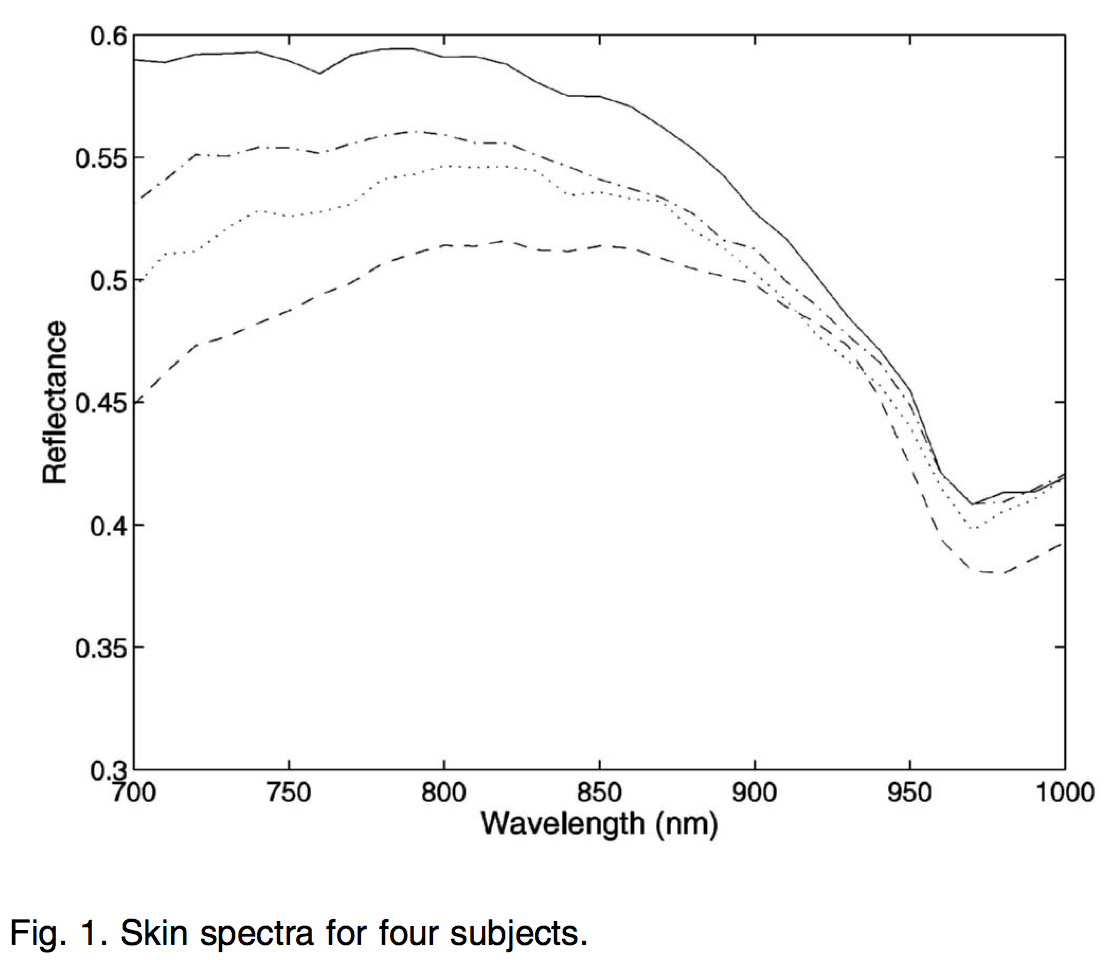
\includegraphics[width=\textwidth]{4subjects}
\end{figure}
\end{column}
\begin{column}{0.5\textwidth}
\begin{figure}
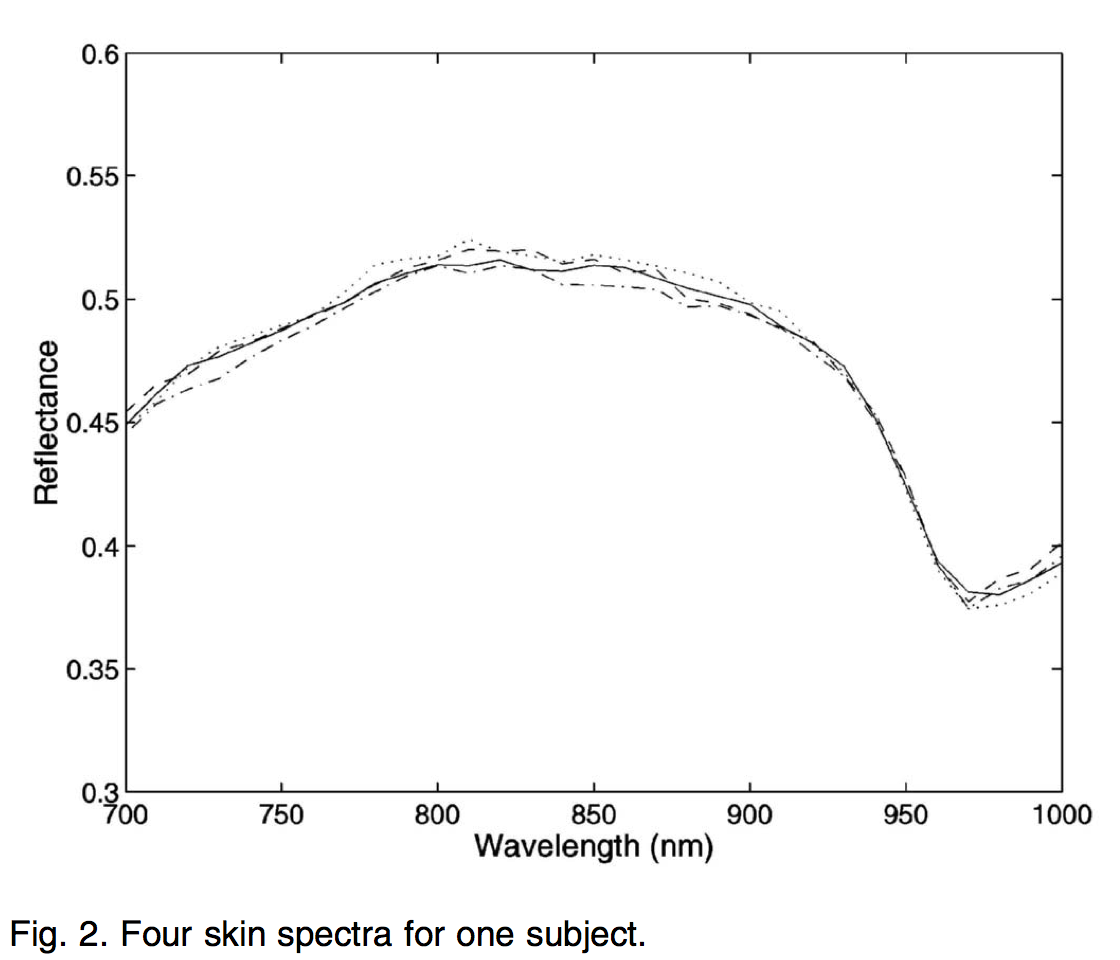
\includegraphics[width=\textwidth]{1subject}
\end{figure}
\end{column}
\end{columns}
\end{frame}

\begin{frame}
\frametitle{Reflectance}
\begin{figure}
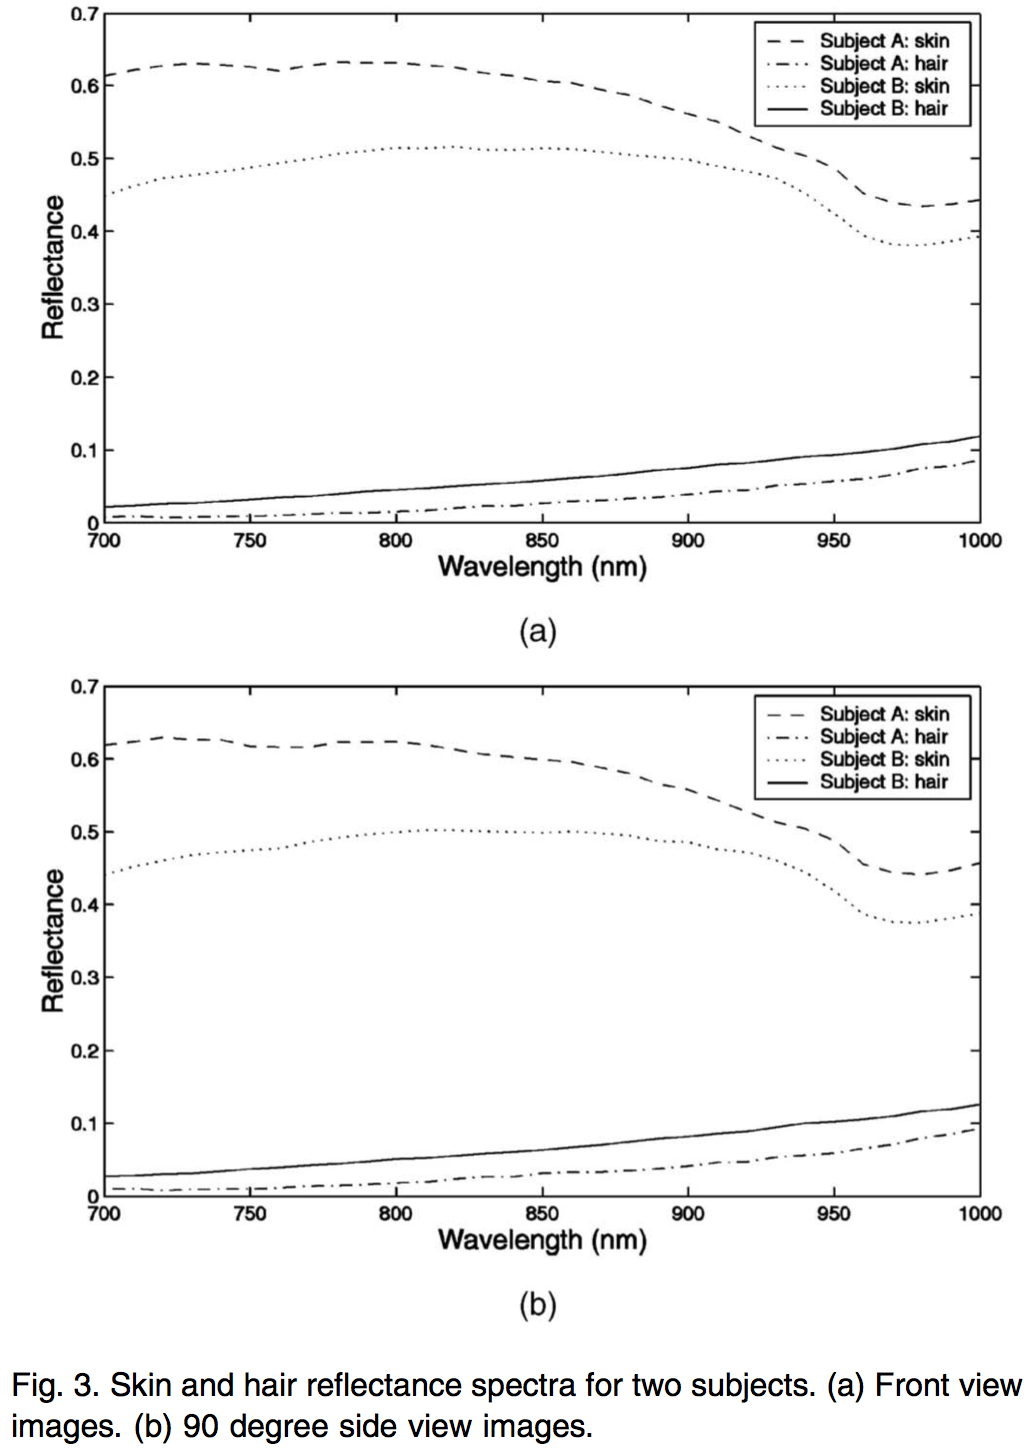
\includegraphics[height=0.8\textheight]{2subjects}
\end{figure}
\end{frame}

\begin{frame}
\frametitle{Data Collection}
\begin{block}{Experimental Setup}
\begin{itemize}
\item 200 subjects
\item 31 spectral bands from 700nm to 1000nm
\item 468x494 spatial resolution
\item 10 second acqusition
\item Two 750W halogen lamps
\item Careful calibration using panels with known reflectance
\end{itemize}
\begin{figure}
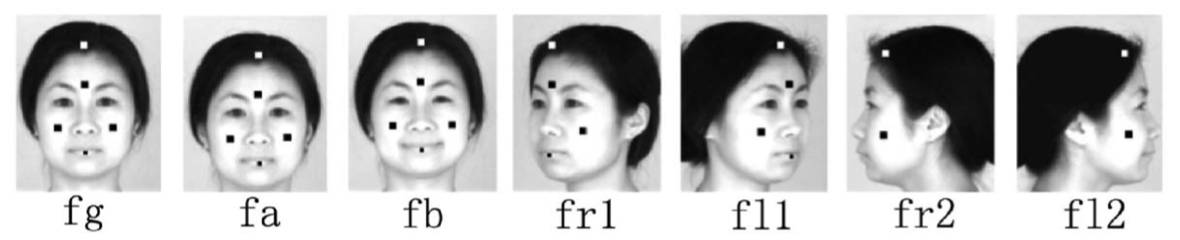
\includegraphics[width=\textwidth]{7poses}
\end{figure}
\end{block}
\end{frame}

\begin{frame}
\frametitle{Representation}
\begin{block}{Enrollment}
\begin{itemize}
\item Manual localization of forehead, cheeks, hair, and lip.
\item For each landmark and channel compute the mean reflectance over a 17x17 block (9x9 for lip).
\item Normalize to unit $L_2$ norm.
\item For each landmark, sample 5 blocks in adjacent locations.
\end{itemize}
\end{block}
\pause
\begin{block}{Comparison}
\begin{itemize}
\item Mahalanobis distance between descriptors, with diagonal covariance matrix.
\item Distance between two landmarks is the minimum of the distance between the $5*5=25$ pairwise descriptors.
\item Distance between faces is the sum of the distances between landmarks.
\end{itemize}
\end{block}
\end{frame}

\begin{frame}
\frametitle{Results}
\begin{figure}
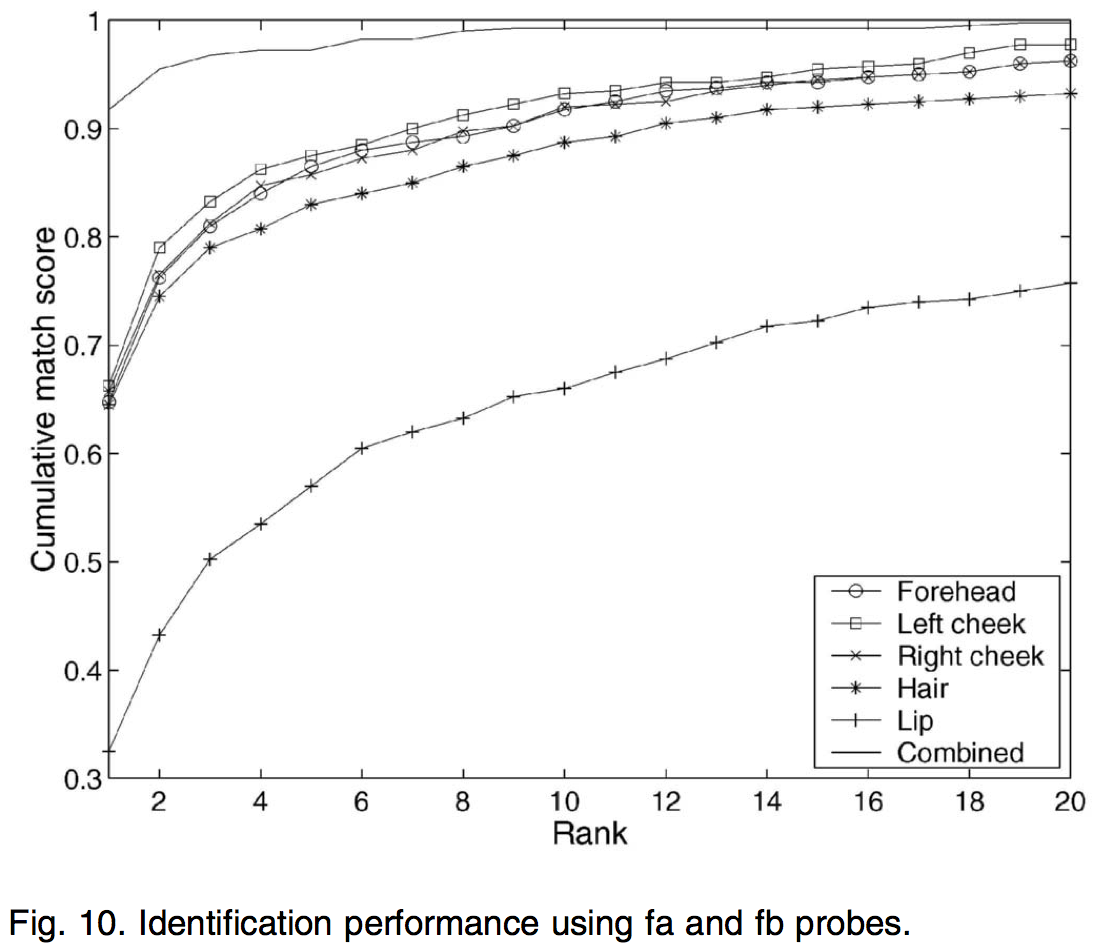
\includegraphics[height=0.8\textheight]{landmarkresults}
\end{figure}
\end{frame}

\begin{frame}
\frametitle{Results}
\begin{figure}
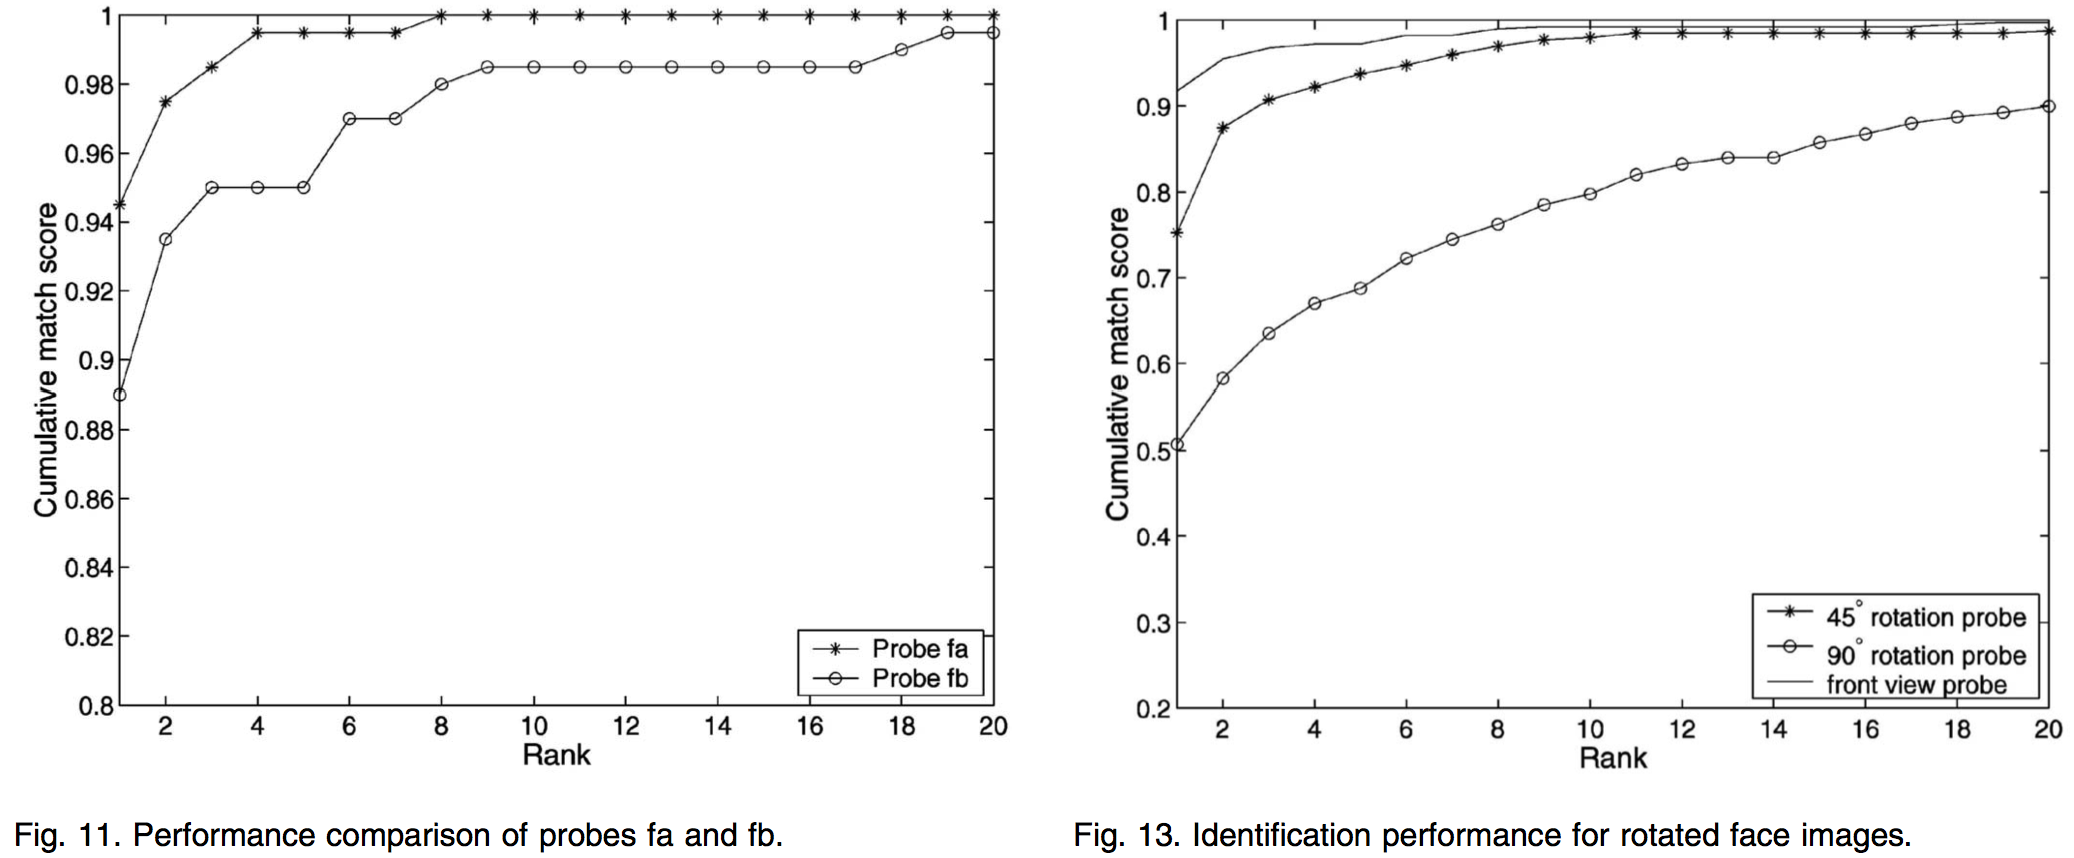
\includegraphics[width=\textwidth]{hyperspectralResults1}
\end{figure}
\end{frame}

\begin{frame}
\frametitle{Results}
\begin{figure}
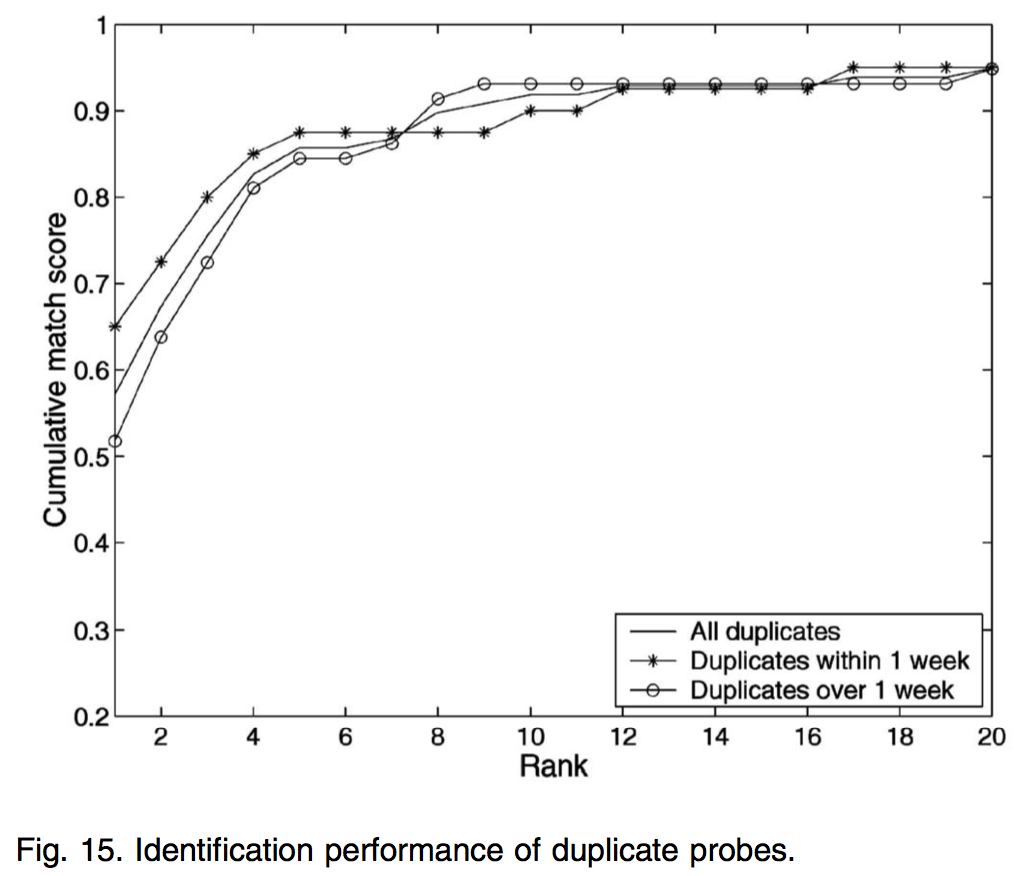
\includegraphics[height=0.8\textheight]{hyperspectralResults2}
\end{figure}
\end{frame}

\section{Thermal}
\begin{frame}
\frametitle{Thermal IR Fusion}
\begin{block}{Abstract}
\begin{itemize}
\item Simultaneously aquired thermal IR and visible light images
\item Two feature level fusion approaches
\item Feature selection using genetic algorithm
\end{itemize}
\end{block}
\pause
\begin{block}{Thermal IR}
\begin{itemize}
\item Strengths
\begin{itemize}
\item illumination
\item expression
\item pose
\item darkness
\end{itemize}
\item Weaknesses
\begin{itemize}
\item temperature changes
\item heat patterns due to physical conditions
\item glass
\end{itemize}
\end{itemize} 
\end{block}
\end{frame}

\begin{frame}
\frametitle{Example Images}
\begin{figure}
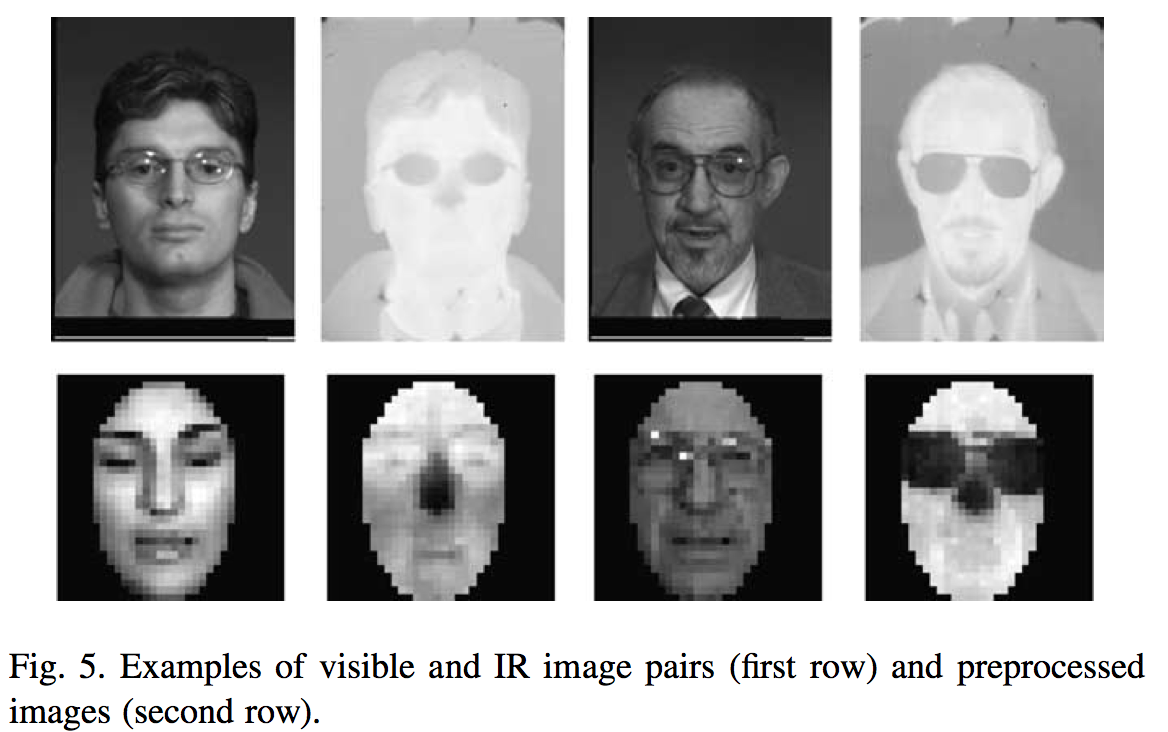
\includegraphics[width=\textwidth]{exampleir}
\end{figure}
\end{frame}

\begin{frame}
\frametitle{Two fusion approaches}
\begin{block}{Pixel-based fusion}
\begin{itemize}
\item Represent both VIS and IR images in a multi-scale Haar wavelet basis
\item Fuse representations by selecting either the VIS or IR coefficient for each wavelet
\item Use GA for coefficient selection
\item Invert the fused representation to reconstruct the face image
\item Apply eigenfaces 
\end{itemize}
\end{block}
\pause
\begin{block}{Feature-based fusion}
\begin{itemize}
\item Apply eigenfaces to learn VIS subspace and IR subspace
\item Fuse representations by selecting either the VIS or IR coefficient for each eigenvector
\item Use GA for coefficient selection
\end{itemize}
\end{block}
\end{frame}

\begin{frame}
\frametitle{Pixel-based fusion}
\begin{figure}
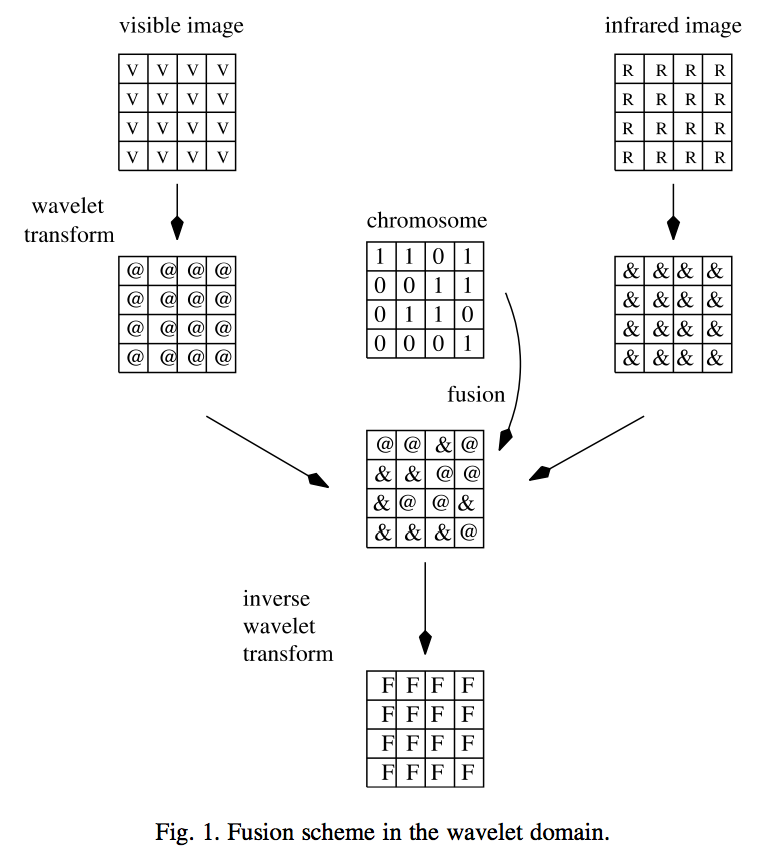
\includegraphics[height=0.8\textheight]{pixelfusion}
\end{figure}
\end{frame}

\begin{frame}
\frametitle{Feature-based fusion}
\begin{figure}
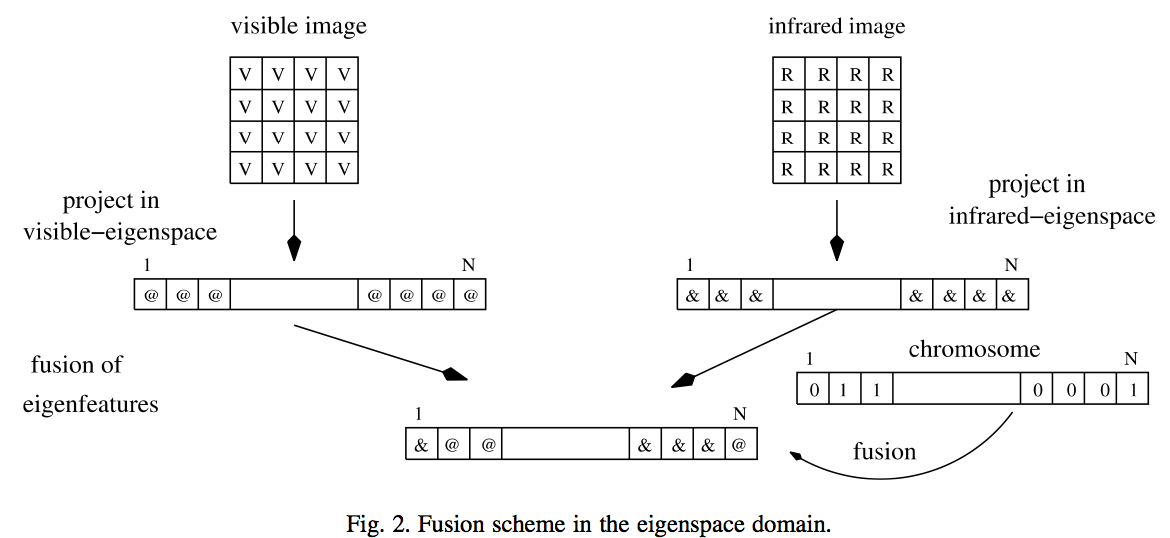
\includegraphics[width=\textwidth]{featurefusion}
\end{figure}
\end{frame}

\begin{frame}
\frametitle{Genetic Search}
\begin{figure}
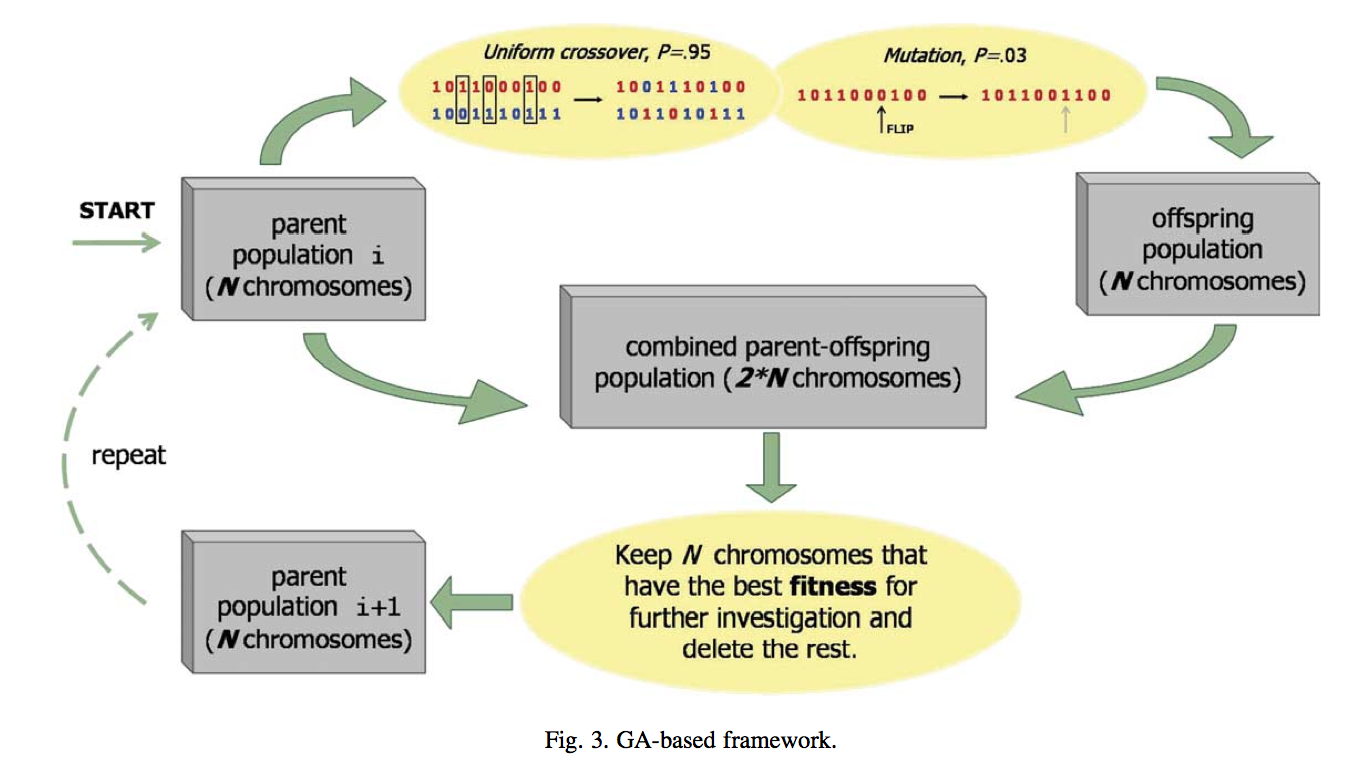
\includegraphics[width=\textwidth]{ga}
\end{figure}
\end{frame}

\begin{frame}
\frametitle{Eyeglasses Results}
\begin{figure}
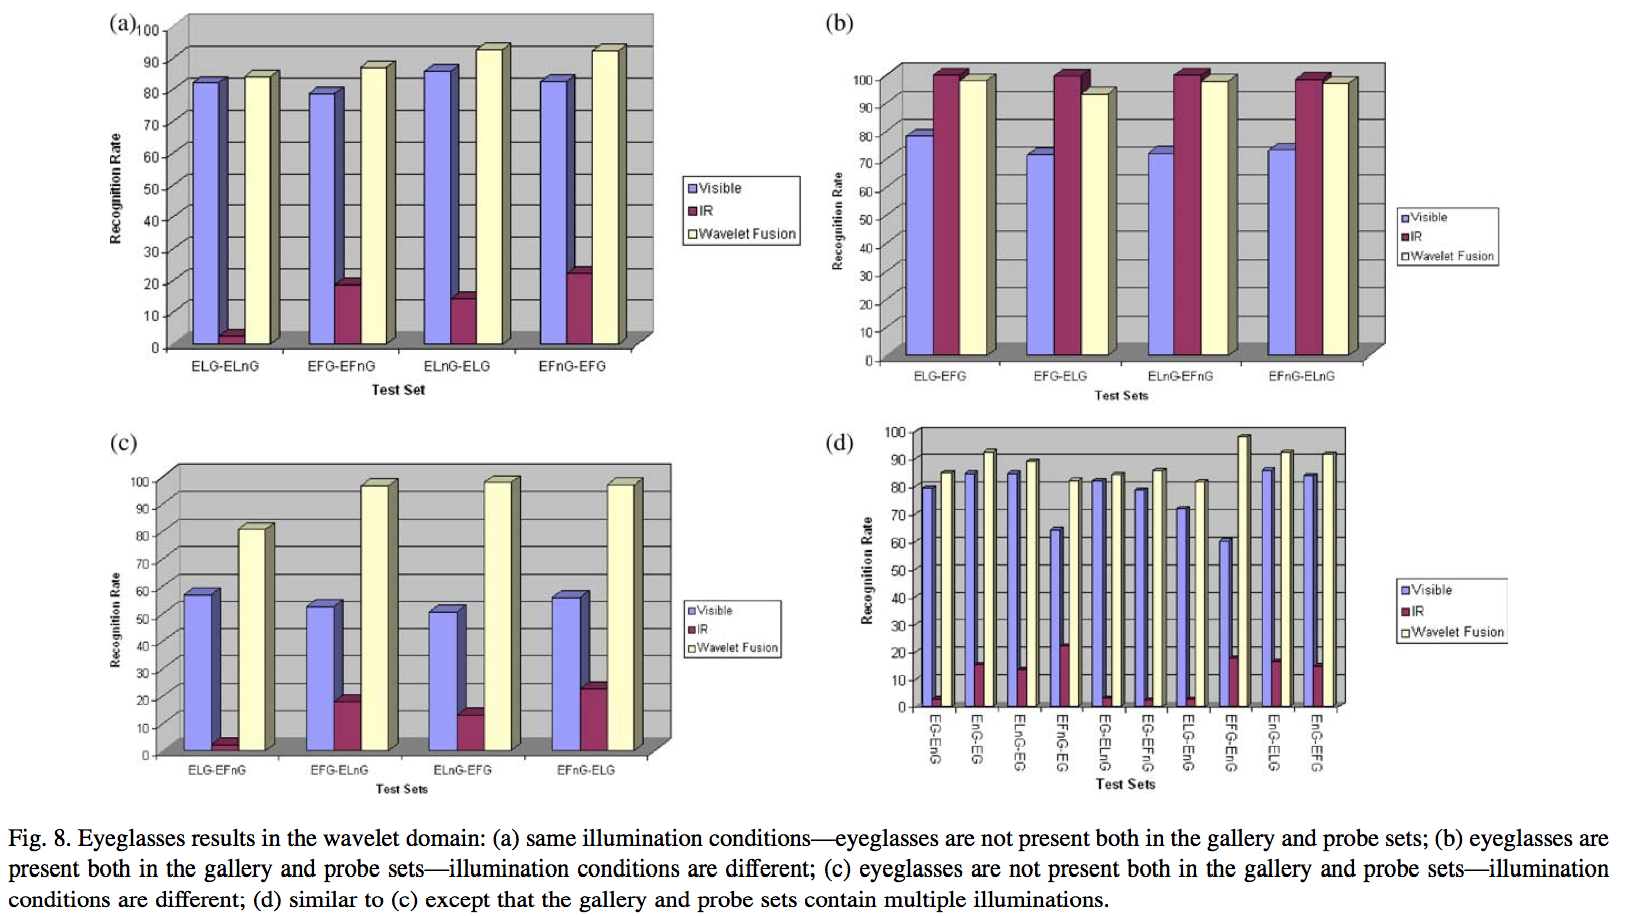
\includegraphics[width=\textwidth]{eyeglassesresults}
\end{figure}
\end{frame}

\begin{frame}
\frametitle{Eyeglasses Results}
\begin{figure}
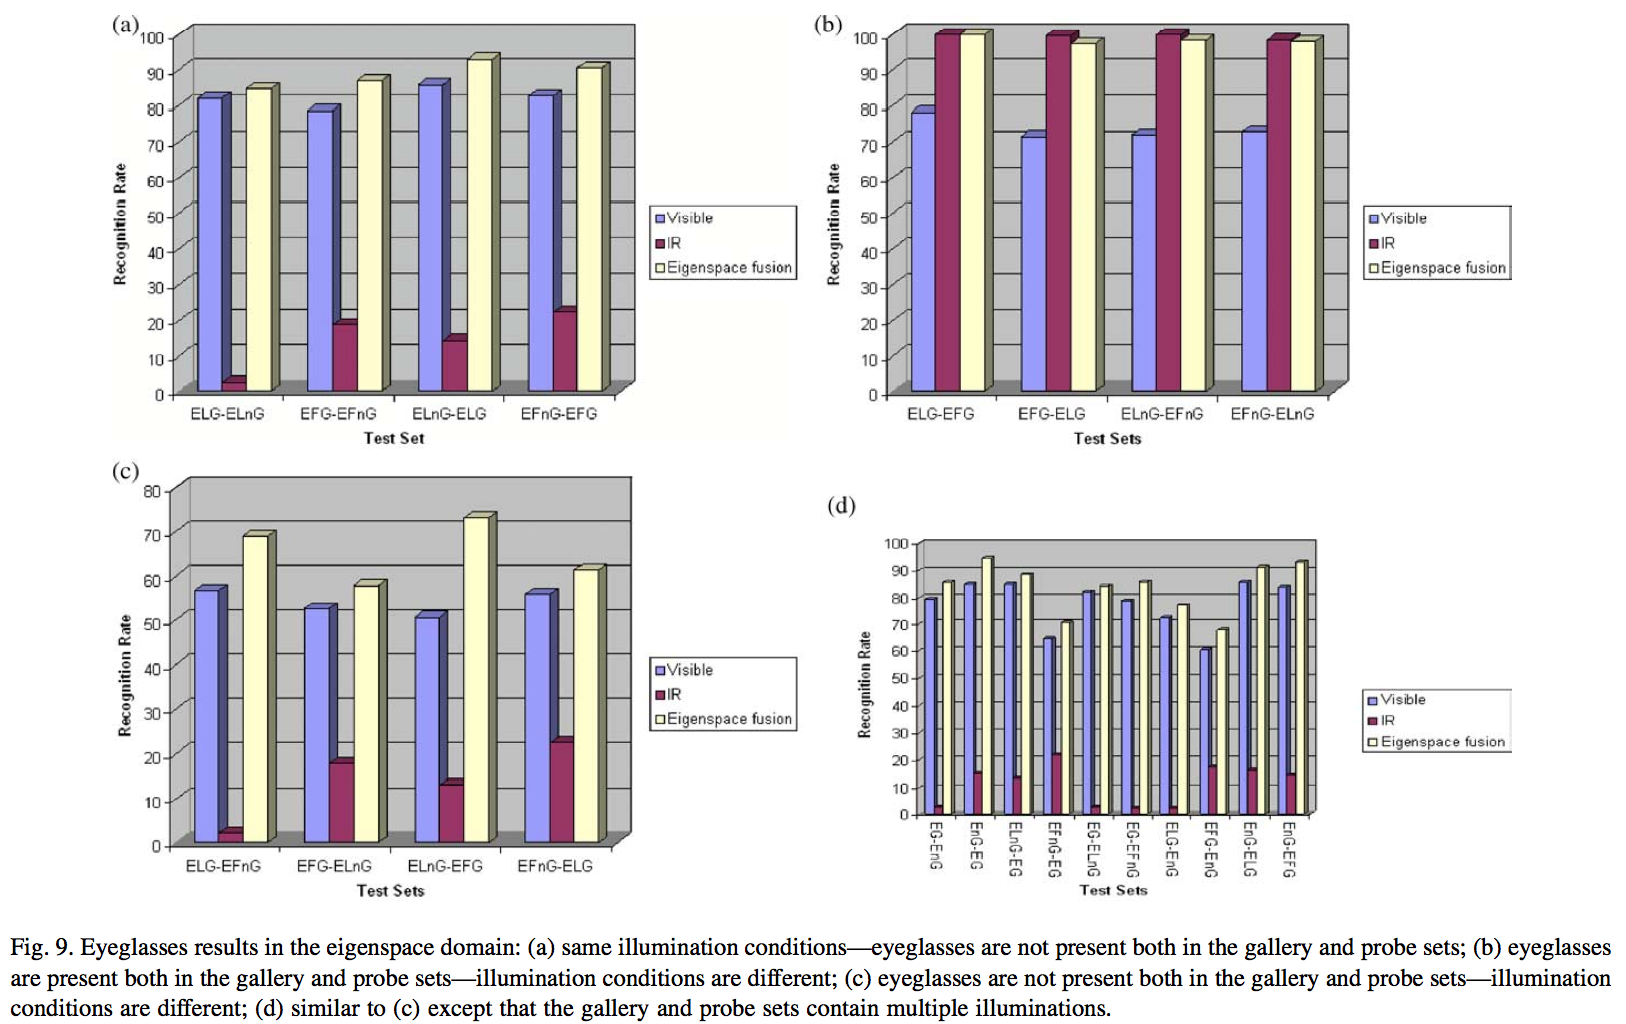
\includegraphics[width=\textwidth]{eyeglassesresults2}
\end{figure}
\end{frame}

\begin{frame}
\frametitle{Expression Results}
\begin{figure}
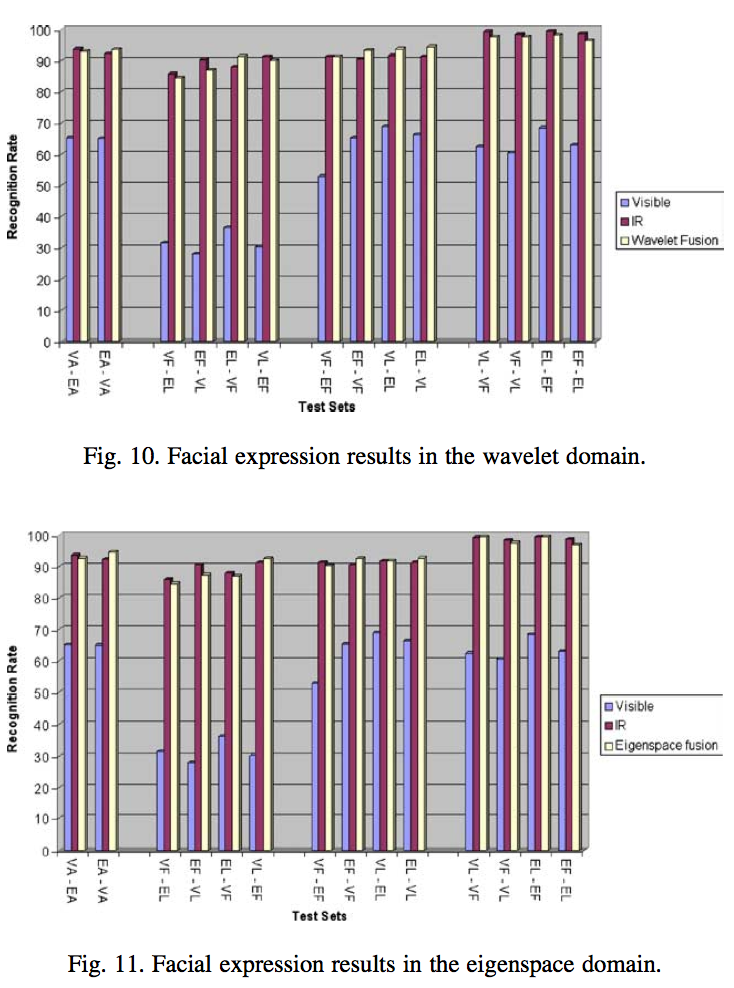
\includegraphics[height=0.8\textheight]{expressionresults}
\end{figure}
\end{frame}

\section{Kernel Prototypes}
\begin{frame}
\frametitle{Kernel Prototypes}
\begin{block}{Abstract}
\begin{itemize}
\item Match across image modalities
\item Process each face using transformations tuned for its modality
\item Represent a face as a vector of similarities to prototype faces
\item Learn a transformation matrix $R$ between gallery and probe prototype spaces
\item Apply LDA using random sampling to overcome small training set size
\end{itemize}
\end{block}
\pause
\begin{block}{Motivation}
\begin{itemize}
\item When a subject's face can only be acquired in nighttime environments.
\item When a verbal description is provided by a witness
\end{itemize}
\end{block}
\end{frame}

\begin{frame}
\frametitle{Four Heterogenous Modalities}
\begin{figure}
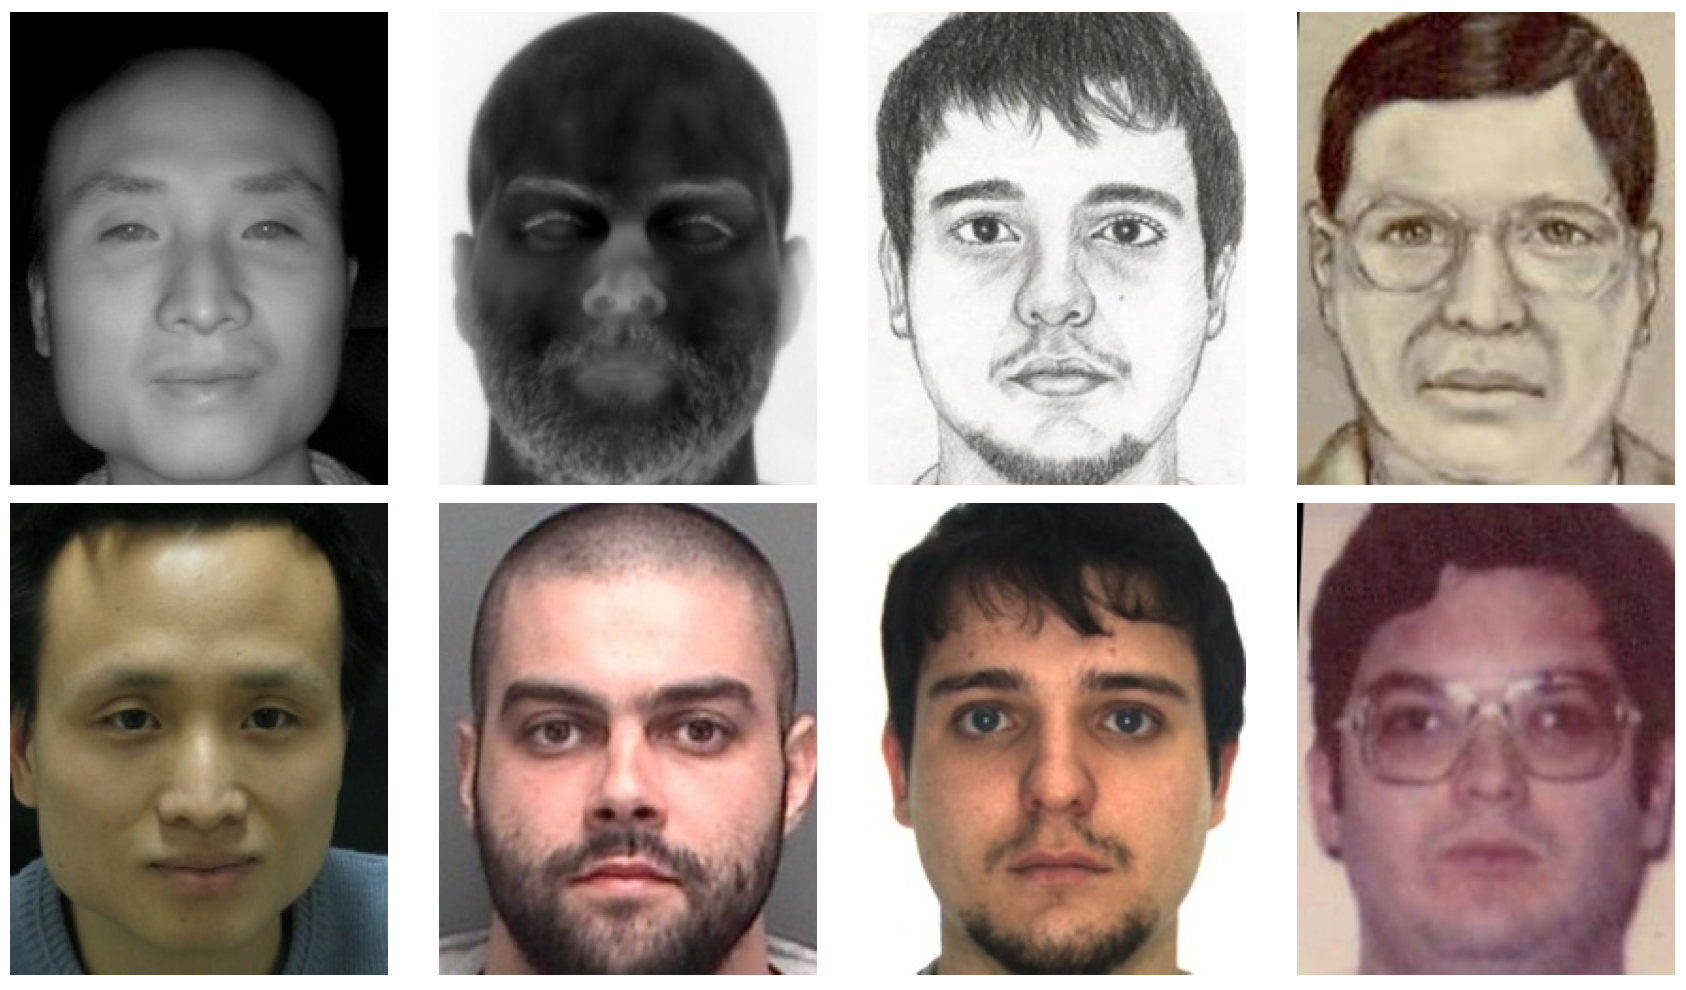
\includegraphics[width=\textwidth]{heterogeneous}
\end{figure}
\end{frame}

\begin{frame}
\frametitle{Feature Extraction}
\begin{figure}
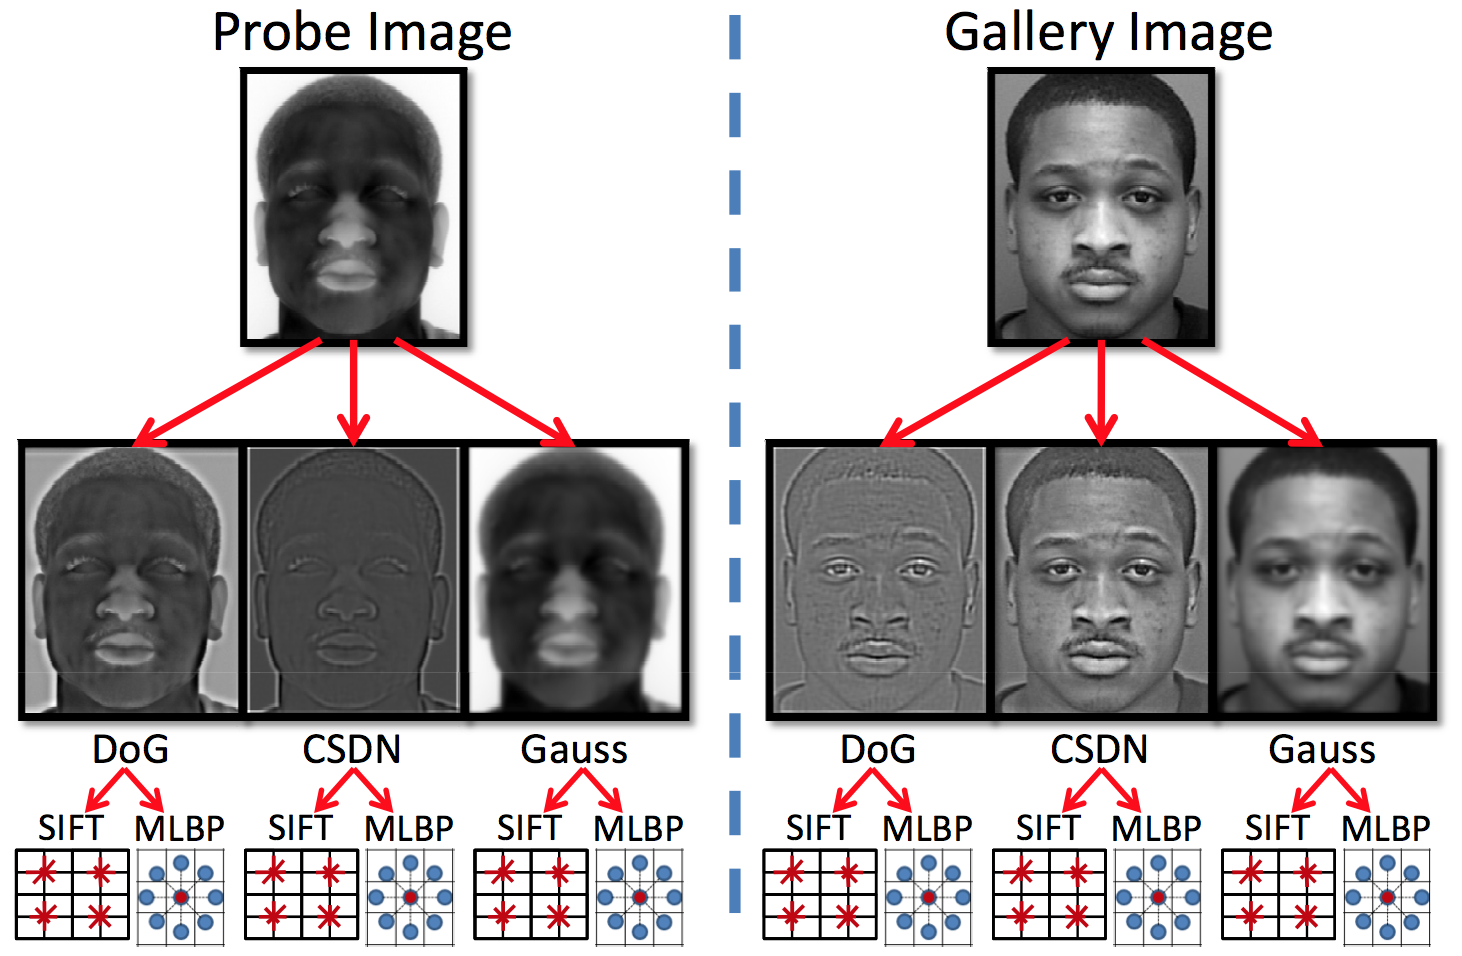
\includegraphics[width=\textwidth]{featureextraction}
\end{figure}
\end{frame}

\begin{frame}
\frametitle{Prototype Representation}
\begin{figure}
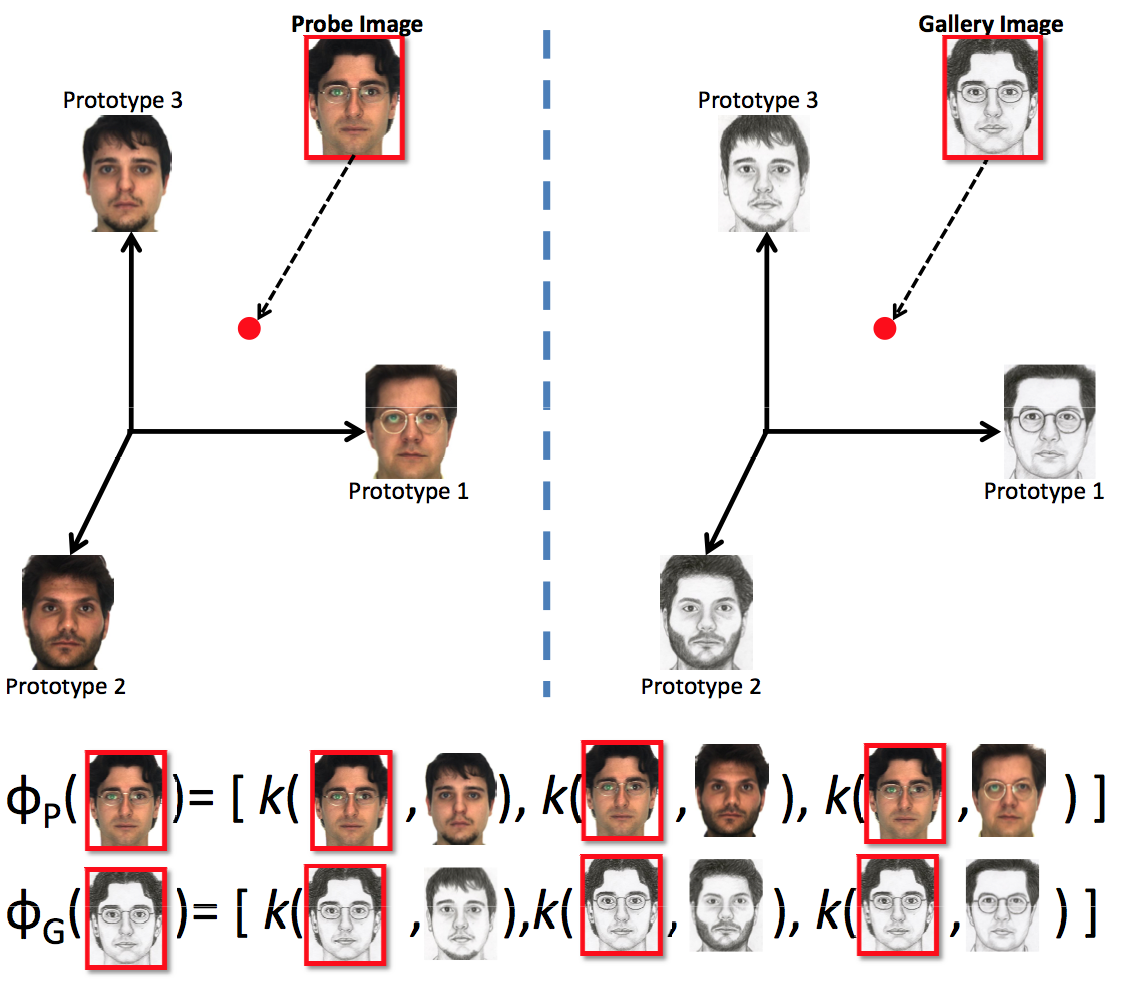
\includegraphics[height=0.8\textheight]{prototypes}
\end{figure}
\end{frame}

\begin{frame}
\frametitle{Math}
\begin{block}{Prototype Framework}
Kernel prototypes
\begin{equation}
\begin{split}
K^P(i,j) &= k(f(P_i), f(P_j)) \\
K^G(i,j) &= k(f(G_i), f(G_j))
\end{split}
\end{equation}
assume
\begin{equation}
k(f(P_i), f(P_j)) \approx k(f(G_i), f(G_j))
\end{equation}
which can be compensated for with
\begin{equation}
R = K^G \cdot (K^P)^{-1}
\end{equation}
to construct a common basis for LDA
\end{block}
\end{frame}

\begin{frame}
\frametitle{Random Sampling}
\begin{figure}
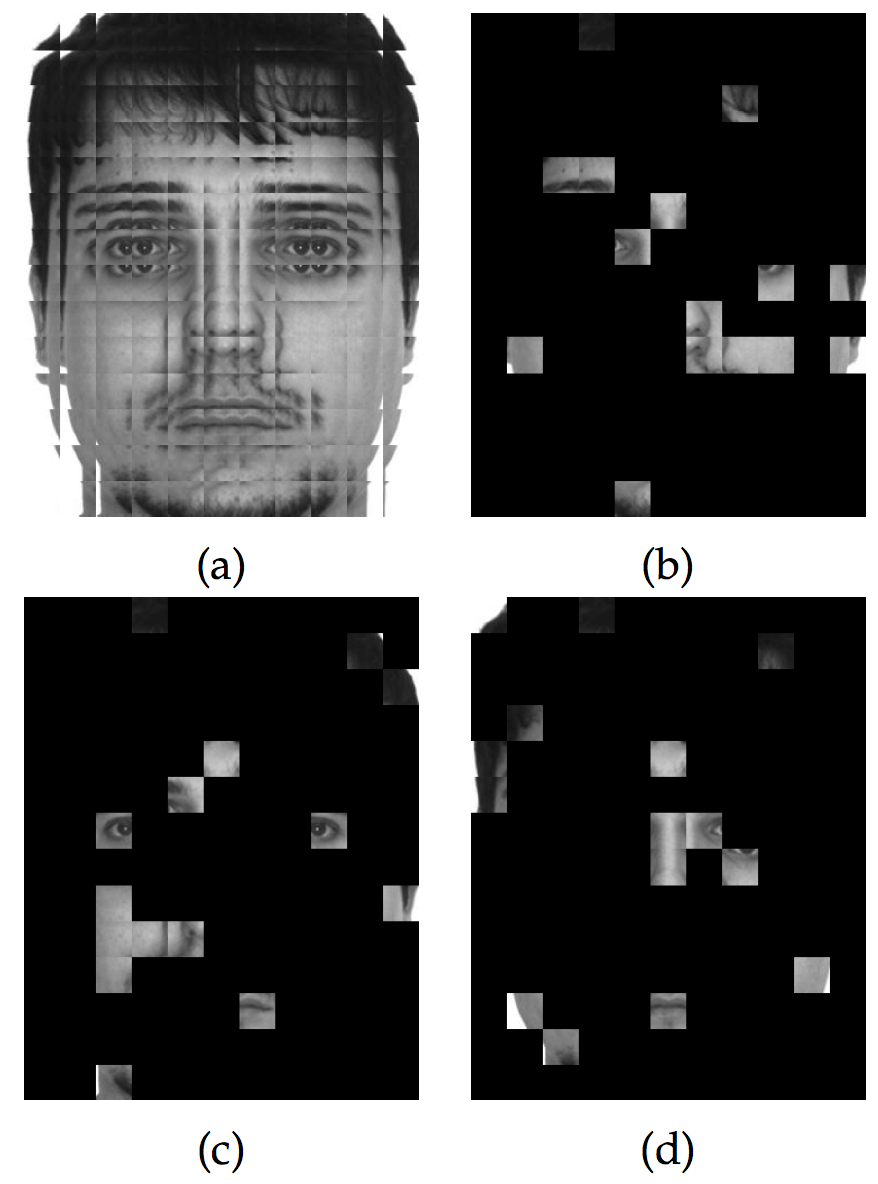
\includegraphics[height=.85\textheight]{randomsampling}
\end{figure}
\end{frame}

\begin{frame}
\frametitle{Results}
\begin{figure}
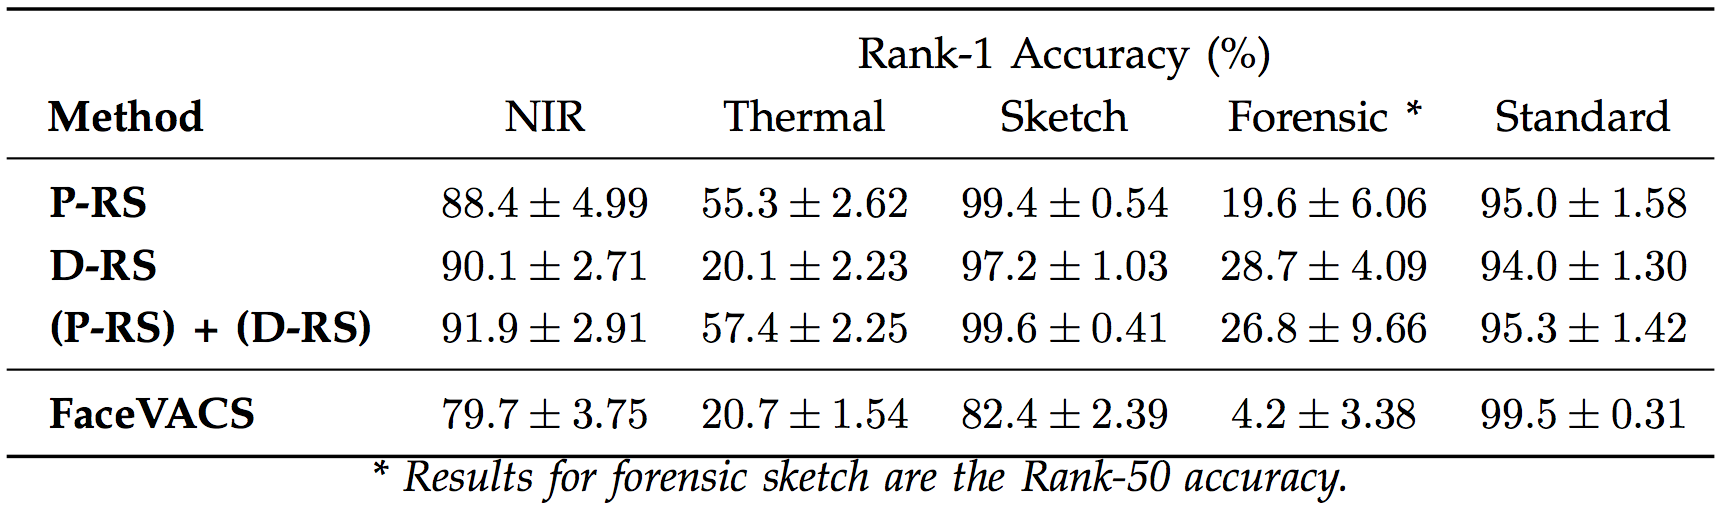
\includegraphics[width=\textwidth]{prototyperesults}
\end{figure}
\end{frame}

\begin{frame}
\frametitle{Results}
\begin{figure}
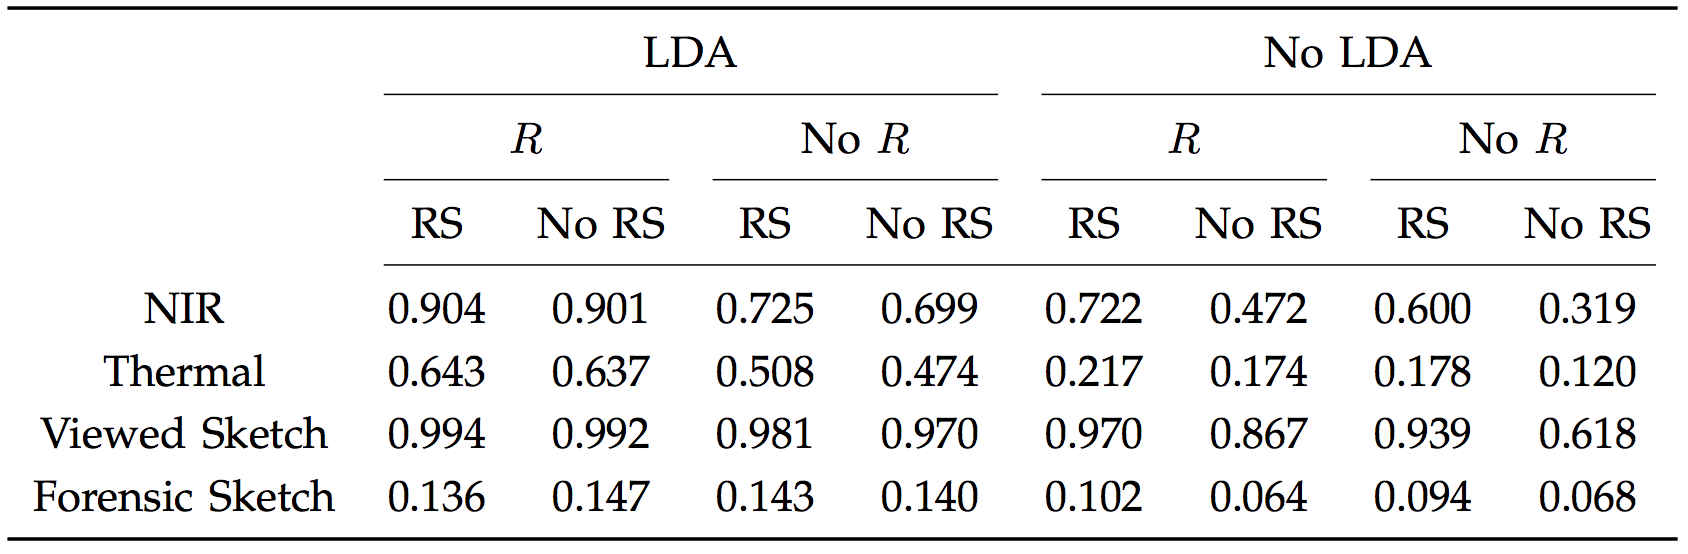
\includegraphics[width=\textwidth]{prototyperesults2}
\end{figure}
\end{frame}

\begin{frame}
\centerline{The End!}
\end{frame}

% End of slides
\end{document}